%%%%%%%%%%%%%%%%%%%%%%%%%%%%%%%%%%%%%%%%%
% Beamer Presentation
% LaTeX Template
% Version 1.0 (10/11/12)
%
% This template has been downloaded from:
% http://www.LaTeXTemplates.com
%
% License:
% CC BY-NC-SA 3.0 (http://creativecommons.org/licenses/by-nc-sa/3.0/)
%
%%%%%%%%%%%%%%%%%%%%%%%%%%%%%%%%%%%%%%%%%

%----------------------------------------------------------------------------------------
%	PACKAGES AND THEMES
%----------------------------------------------------------------------------------------

\documentclass{beamer}
\usepackage[latin1]{inputenc}
\usepackage{multirow}
\usepackage{amsmath}

\mode<presentation> {

% The Beamer class comes with a number of default slide themes
% which change the colors and layouts of slides. Below this is a list
% of all the themes, uncomment each in turn to see what they look like.

%\usetheme{default}
%\usetheme{AnnArbor}
%\usetheme{Antibes}
%\usetheme{Bergen}
%\usetheme{Berkeley}
%\usetheme{Berlin}
%\usetheme{Boadilla}
%\usetheme{CambridgeUS}
%\usetheme{Copenhagen}
%\usetheme{Darmstadt}
%\usetheme{Dresden}
%\usetheme{Frankfurt}
%\usetheme{Goettingen}
%\usetheme{Hannover}
%\usetheme{Ilmenau}
%\usetheme{JuanLesPins}
%\usetheme{Luebeck}
\usetheme{Madrid}
%\usetheme{Malmoe}
%\usetheme{Marburg}
%\usetheme{Montpellier}
%\usetheme{PaloAlto}
%\usetheme{Pittsburgh}
%\usetheme{Rochester}
%\usetheme{Singapore}
%\usetheme{Szeged}
%\usetheme{Warsaw}

% As well as themes, the Beamer class has a number of color themes
% for any slide theme. Uncomment each of these in turn to see how it
% changes the colors of your current slide theme.

%\usecolortheme{albatross}
%\usecolortheme{beaver}
%\usecolortheme{beetle}
%\usecolortheme{crane}
%\usecolortheme{dolphin}
%\usecolortheme{dove}
%\usecolortheme{fly}
%\usecolortheme{lily}
%\usecolortheme{orchid}
%\usecolortheme{rose}
%\usecolortheme{seagull}
%\usecolortheme{seahorse}
%\usecolortheme{whale}
%\usecolortheme{wolverine}

%\setbeamertemplate{footline} % To remove the footer line in all slides uncomment this line
%\setbeamertemplate{footline}[page number] % To replace the footer line in all slides with a simple slide count uncomment this line

%\setbeamertemplate{navigation symbols}{} % To remove the navigation symbols from the bottom of all slides uncomment this line
}

\usepackage{graphicx} % Allows including images
\usepackage{booktabs} % Allows the use of \toprule, \midrule and \bottomrule in tables

%----------------------------------------------------------------------------------------
%	TITLE PAGE
%----------------------------------------------------------------------------------------

\title[JCHARMING]{JCHARMING: A Bug Reproduction Approach using Crash Traces and Directed Model Checking} % The short title appears at the bottom of every slide, the full title is only on the title page

\author[Mathieu Nayrolles]{\underline{Mathieu Nayrolles$^1$}, Wahab Hamou-Lhadj$^1$, Sofi\`ene Tahar$^2$ and Alf Larsson$^3$} % Your name
\institute[Concordia] % Your institution as it will appear on the bottom of every slide, may be shorthand to save space
{
$^1$Software Behaviour Analysis (SBA) Research Lab, ECE,  Concordia, Montr\'eal, Canada\\
$^2$Hardware Verification Group (HVG) Research Lab, ECE, Concordia, Montr\'eal, Canada \\ 
$^3$PLF System Management, R\&D Ericsson, Stockholm, Sweden \\ 
\medskip
\textit{mathieu.nayrolles@gmail.com, wahab.hamou-lhadj@concordia.ca, tahar@ece.concordia.ca, alf.larsson@ericsson.com} % Your email address
}
\date{March 4, 2015} % Date, can be changed to a custom date

\begin{document}

\begin{frame}
\titlepage % Print the title page as the first slide
\end{frame}


\begin{frame}
\frametitle{Context: Software are released with bugs.}

\begin{itemize}
\item Despite testing and verification, softwares are pledged to be released with latent bugs.
\vspace{0.3cm}
\item Latent bugs will cause field crashes / faillures.
\vspace{0.3cm}
\item Patching field faillures is challenging:
\begin{itemize}
\vspace{0.3cm}
\item We have to know about them.
\vspace{0.3cm}
\item Information is scarce and inconsistent
\vspace{0.3cm}
\item Most valuable information are the one that help to reproduce a bug [Bettenburg, 2008].
\end{itemize}
\end{itemize}
\end{frame}

\begin{frame}
\frametitle{Related Works: Current ways to reproduce a crash.}
\begin{columns}[c] % The "c" option specifies centered vertical alignment while the "t" option is used for top vertical alignment

\column{.45\textwidth} % Left column and width
\textbf{Record and replay}
\begin{itemize}
\item Instrumentation of source code
\item Record on-field execution
\item Replay in-house
\vspace{0.3cm}
\item Cheap \& easy to implement
\item Yield good results
\item Overhead (1\% to 1066\%) and privacy concerns
\vspace{0.3cm}
\item JRapture'00, BugNet'05, ReCrash'08
\end{itemize}


\column{.5\textwidth} % Left column and width

\textbf{In house crash reproduction}
\begin{itemize}
\item Core dump.
\item Forward Symbolic Execution.
\item Backward Symbolic Execution.
\vspace{0.3cm}
\item Yield average results.
\item NP-Compex Problem
\item Exponential learning curve.
\item Privacy concerns.
\vspace{0.3cm}
\item BugRedux'12, RECORE'13, STAR'13
\end{itemize}

\end{columns}
\end{frame}


%------------------------------------------------


\begin{frame}
\frametitle{JCHARMING: A different direction}
\begin{itemize}

\item Avoid code instrumentation
\begin{itemize}
\vspace{0.3cm}
\item 0\% overhead
\end{itemize}
\vspace{0.3cm}
\item Do no yield privacy concerns
\begin{itemize}
\vspace{0.3cm}
\item Scalable to real-world and industrial/proprietary software systems
\end{itemize}
\vspace{0.3cm}
\item Leverage the stack traces resulting from a crash
\begin{itemize}
\vspace{0.3cm}
\item More and more often present in bug reports
\end{itemize}
\vspace{0.3cm}
\item JCHARMING uses directed model checking and backward slicing.
\end{itemize}
\end{frame}

%------------------------------------------------

\begin{frame}
\frametitle{Prelimenaries: Model Checking}

\begin{itemize}

\item Checks if a given system under test (SUT) meets a specification $p$ by exhaustively testing every states. [Visser, 2003], [Kropf, 1999]

\item Generates a counter example if $p$ cannot be met.

\item Represented by a Kripke structure [Kripke, 1963]:
\end{itemize}

\begin{center}
$SUT = < S, T, P >$ ,  $(SUT, x) \models p$
\end{center}

\begin{itemize}

\item Ensures that $p$ is reached at some point and not that $p$ holds nor $\forall x, p$ is satisfiable.
\item In JCHARMING, we aim to verify that $\forall$ states the program does not crash:

\end{itemize}

\begin{center}
$\forall x.(SUT, x) \models \neg c$
\end{center}


\end{frame}

%------------------------------------------------

\begin{frame}
\frametitle{Prelimenaries: \textbf{Testing}, Model Checking and Directed Model Checking}

\begin{figure}
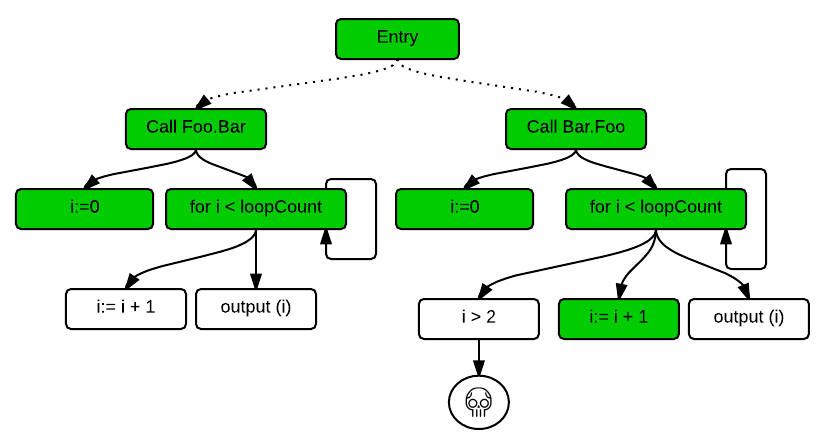
\includegraphics[width=0.75\linewidth]{media/test.png}
\end{figure}
\begin{itemize}
\item Depends on the tester understanding of the SUT.
\item Ineficient because it is not exhaustive.
\end{itemize}

\end{frame}

\begin{frame}
\frametitle{Prelimenaries: Testing, \textbf{Model Checking} and Directed Model Checking}

\begin{figure}
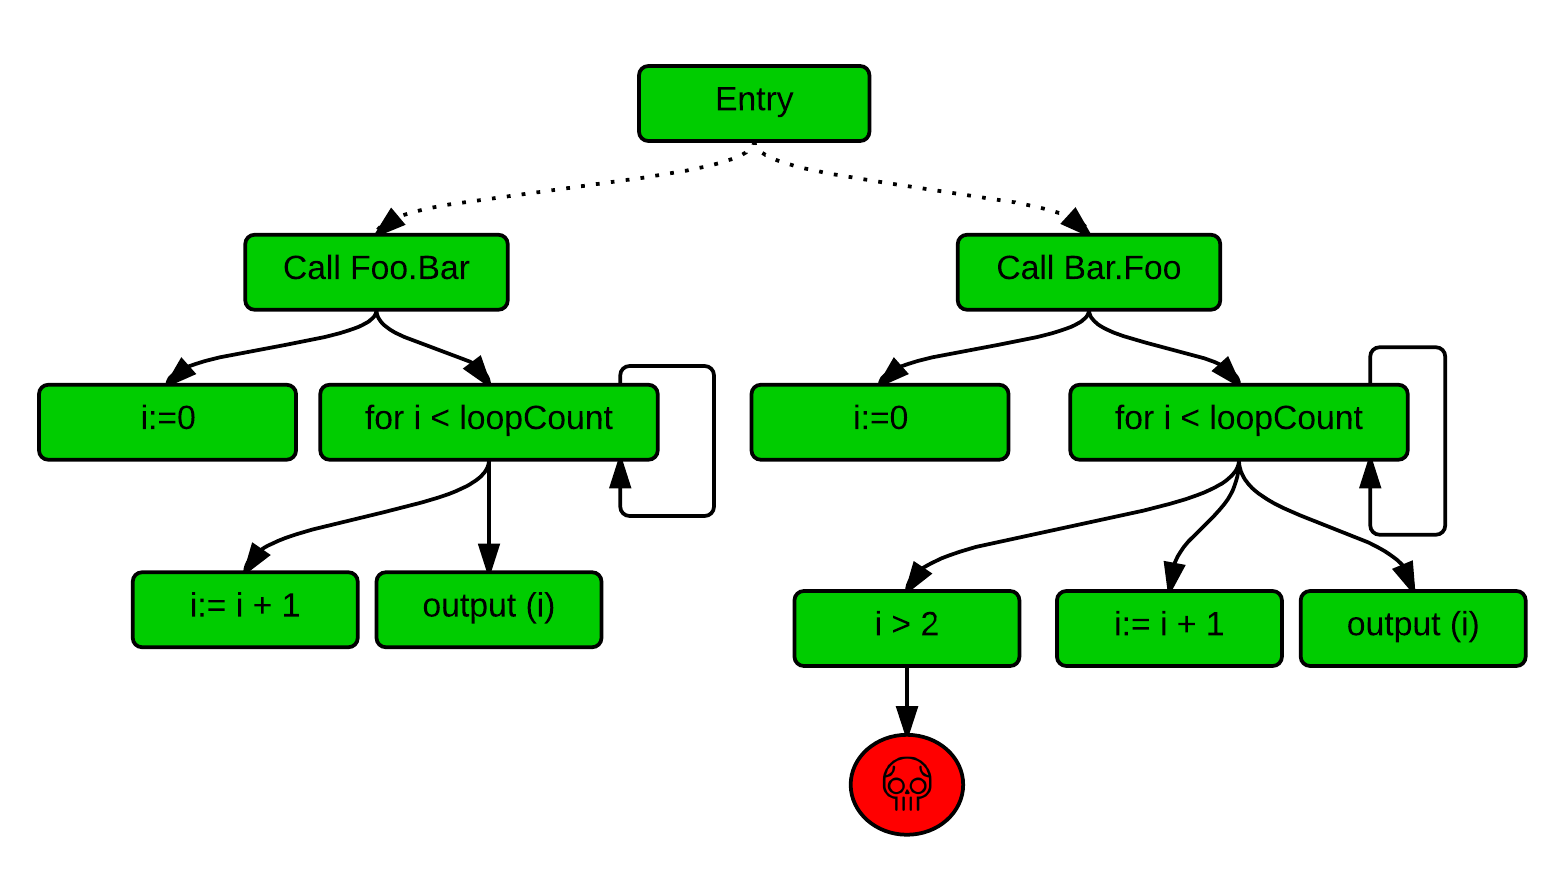
\includegraphics[width=0.75\linewidth]{media/mc.png}
\end{figure}

\begin{itemize}
\item Explores each and every state of the program, hence it is complete.
\item Impractical for real-world and large systems
\end{itemize}

\end{frame}


\begin{frame}
\frametitle{Prelimenaries: Testing, Model Checking and \textbf{Directed Model Checking}}

\begin{figure}
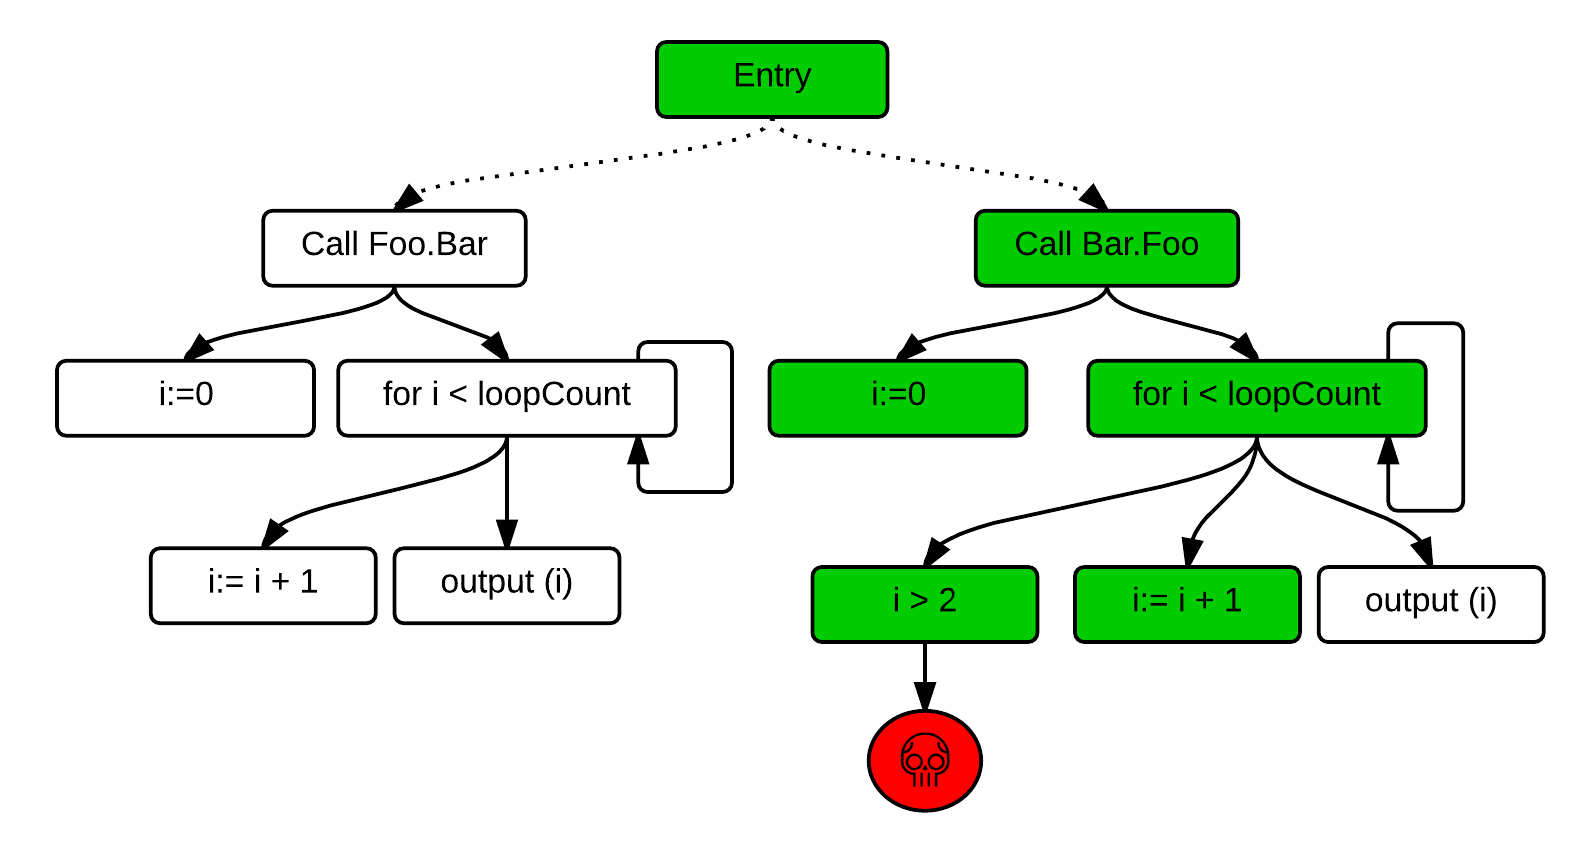
\includegraphics[width=0.75\linewidth]{media/dmc.png}
\end{figure}

\begin{itemize}
\item Explores only the states that may lead to a
specific location. [Rungta, 2009]
\item Use insights -- generally heuristics -- about the SUT to prune states.
\end{itemize}

\end{frame}

\begin{frame}
\frametitle{The JCHARMING approach}

\begin{figure}
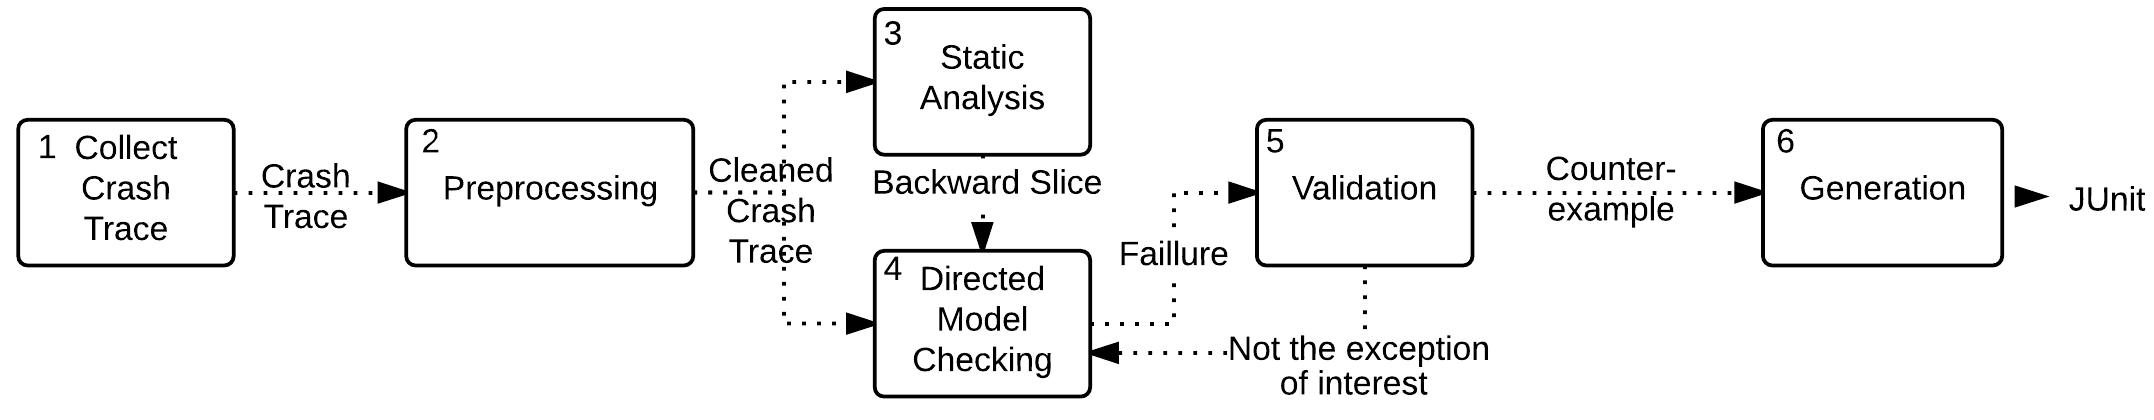
\includegraphics[width=0.97\linewidth]{media/approach.png}
\end{figure}

\begin{itemize}
\item \textbf{Step 1: Collect the crash trace}

\begin{small}
\texttt{1.javax.activity.IAE:loopTimes
should be < 3\\
2. at Foo.bar(Foo.java:10)\\
3. at GUI.buttonActionPerformed(GUI.java:88)\\
4. at GUI.access\$0(GUI.java:85)\\
5. at GUI\$1.actionPerformed(GUI.java:57)\\
6. caused by java.lang.IndexOutOfBoundsException : 3\\
7. at saner.Foo.buggy(Foo.java:17)\\
8. and 4 more ...\\}
\end{small}

\item \textbf{Step 2: Preprocessing}

\end{itemize}

\end{frame}

\begin{frame}
\frametitle{Step 3: Building the Backward Static Slice}

\begin{itemize}
\item Large systems does not necessary contain all
the methods that have been executed starting from the entry
point of the program to the crash [Oracle, 2011]
\item We need to complete the missing frames of the stack traces
\item A backward slice contains all possible branches that may lead to a point $n$ from a point $m$ as well as the definition of the variables that control these branches
\item We perform a static backward slice between each frame to
compensate for possible missing information in the crash
trace:

\begin{center}
$ bslice_{[entry \leftarrow f_0]} = bslice_{[f_1 \leftarrow f_0]} \cup ... \cup bslice_{[entry \leftarrow f_n]}$
\end{center}

\end{itemize}

\end{frame}

\begin{frame}
\frametitle{Step 3: Building the Backward Static Slice (Cont'd)}

\begin{columns}[c] % The "c" option specifies centered vertical alignment while the "t" option is used for top vertical alignment

\column{.60\textwidth} % Left column and width
\begin{itemize}

\item The union of the sub backward static slices is a subset of the backward static slice from $f_0$ to entry.

\begin{center}
$\bigcup_{i=0}^{entry} bslice_{[f_{i+1} \leftarrow f_i]} \subseteq bslice_{[f_{entry} \leftarrow f_0]}$ 
\end{center}
\vspace{0.5cm}
\item If $z_2$ is a prerequisite to $f_2$:
\begin{itemize}
\item $bslice_{[f_{entry} \leftarrow f_0]} = \{f_0, f_1, f_2, z_0, z_1, z_2, z_3\}$
\vspace{0.3cm}
\item $\bigcup_{i=0}^{entry} bslice_{[f_{i+1} \leftarrow f_i]} = \{f_0, f_1, f_2, z_2\}$
\end{itemize}

\end{itemize}

\column{.4\textwidth} % Left column and width

\begin{figure}
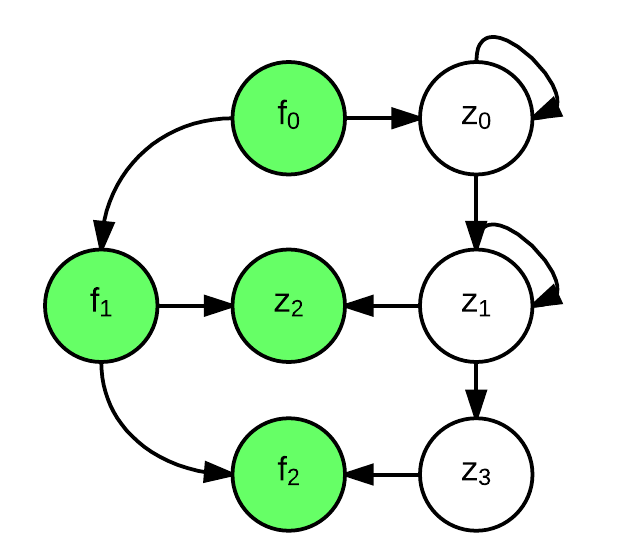
\includegraphics[width=0.95\linewidth]{media/slices.png}
\end{figure}

\end{columns}


\end{frame}

\begin{frame}
\frametitle{Step 3: Building the Backward Static Slice (Cont'd)}

\begin{itemize}
\item The search space for the model checker is limited by the backward slice:
\vspace{0.3cm}
\begin{center}

$ \exists x. 
  \begin{pmatrix}
   \bigcup_{i=0}^{entry} bslice_{[f_{i+1} \leftarrow f_i]} \, \subset \, SUT \\
   $
   $x.\bigcup_{i=0}^{entry} bslice_{[f_{i+1} \leftarrow f_i]} \, \subset \, x.SUT \\
  \end{pmatrix}
  \models c_{i > 2}
 $

\end{center}
\vspace{0.7cm}
\item It exists a sequence of states transitions $x$ that satisfies $c_{i > 2}$ in  $\bigcup_{i=0}^{entry} bslice_{[f_{i+1} \leftarrow f_i]}$

\end{itemize}


\end{frame}

\begin{frame}
\frametitle{Step 4: Directed Model Checking}

\begin{itemize}

\item We use Java PathFinder (JPF)
\begin{itemize}
\item JVM for Java bytecode verification.
\item Front-end for the SPIN model checker.
\item Developped and maintained by NASA.
\end{itemize}



\item Generate states
\item Forward

\begin{itemize}
\item Generates the next state $S_{t+1}$ and add it to the backtrack table
\end{itemize}

\item Backward

\item Backtrack
\begin{itemize}
\item Restore the last state of the backtrack table.
\end{itemize}

\item Restore state

\item Check properties

\begin{itemize}
\item Is triggered after each forward, backward and restore operations.
\end{itemize}


\end{itemize}

\end{frame}

\begin{frame}
\frametitle{Step 4: Directed Model Checking (Cont'd)}

\begin{itemize}


\item We modified the \textit{generate states} and the \textit{forward steps}.
\item The \textit{generate states} is populated with:
\vspace{0.3cm}
\begin{center}
$\bigcup_{i=0}^{entry} bslice_{[f_{i+1} \leftarrow f_i]} \, \subset \, SUT$
\end{center}
\vspace{0.3cm}
\item The \textit{foward step} can explore a state if $s_{i+1}$ and the transition $x$ from $s_i$ to $s_{i+1}$ are in 

\begin{center}
 $\begin{pmatrix}
   \bigcup_{i=0}^{entry} bslice_{[f_{i+1} \leftarrow f_i]} \, \subset \, SUT \\
   $
   $x.\bigcup_{i=0}^{entry} bslice_{[f_{i+1} \leftarrow f_i]} \, \subset \, x.SUT \\
  \end{pmatrix}$
\end{center}
\vspace{0.3cm}
\item JPF is now directed and explores only a sub-system of the SUT.
\end{itemize}

\end{frame}


\begin{frame}
\frametitle{Step 5: Verification}

\begin{itemize}

\item We modify the \textit{check properties} step of JPF:

\begin{itemize}
\item If the current states transitions $x$ yield an exception
\item We execute $x$ and compare the stack trace to the original
\item If the two exceptions match, the bug is \textit{reproduced}.
\end{itemize}

\vspace{0.3cm}

\item Bug can be partially reproduced if the generated exception matches the original by a factor of $t$:

\begin{itemize}
\item Same faillure can be reached by different paths. [Kim, 2013]
\item Might enhance the comprehension.
\item Might speed-up the deployment of a fix.
\end{itemize}

\end{itemize}

\end{frame}


\begin{frame}
\frametitle{Step 6: Generating Test Cases for Bug Reproduction}

\begin{itemize}
\item A JUnit test suite allows developers to reproduce the bug on the press of a button
\vspace{0.3cm}
\item JPF keeps track of the visited states during the model checking process.
\vspace{0.3cm}
\item We leverage this ability to create the required objects and call the methods leading to the crash.
\end{itemize}



\end{frame}



\begin{frame}
\frametitle{Experiments}
\begin{itemize}

\item Aim to answer the following RQ: \textit{Can we use
crash traces and directed model checking to reproduce on-field bugs in a reasonable amount of time?}

\item Randomly selected 1 from 10 bugs containing a stack trace for each system

\begin{table}[h]
\begin{tabular}{llrl}
\hline
SUT        & KLOC & NoC                      & Bug \#ID                                                                                  \\ \hline
Ant        & 265  & 1233                     & 38622, 41422                                                                              \\
ArgoUML    & 58   & 1922                     & 2603, 2558, 311, 1786                                                                     \\
dnsjava    & 33   & 182                      & 38                                                                                        \\
jfreechart & 310  & 990                      & 434, 664, 916                                                                             \\
Log4j      & 70   & 363                      & \begin{tabular}[c]{@{}l@{}}11570, 40212, 41186, 45335,\\ 46271, 47912, 47957\end{tabular} \\
MCT        & 203  & \multicolumn{1}{l}{1267} & 440ed48                                                                                   \\
pdfbox     & 201  & \multicolumn{1}{l}{957}  & 1412, 1359                                                                                \\ \hline
\end{tabular}
\end{table}


\end{itemize}
\end{frame}

\begin{frame}
\frametitle{Experiments (Cont'd)}
\begin{itemize}
\item 85\% success ratio (17/20) with $t = 80\%$
\item 16 minutes average time to reproduce.
\end{itemize}
\begin{table}[h]
\begin{tabular}{l|l}
\hline
SUT        & Bug \#ID                                                                                                                                    \\ \hline
Ant        & \textbf{38622 (25.4m)}, 41422 (-)                                                                                                                    \\ \hline
ArgoUML    & 2603 (9.4m), 2558 (10.6m), \textbf{311 (11.3m)} , 1786 (9.9m)                                                                                        \\ \hline
dnsjava    & \textbf{38 (4m)                                                                                                                                    } \\ \hline
jfreechart &\textbf{ 434 (27.3m)}, 664 (31.2m) , \textbf{916 (26.4m)                                                                                                     } \\ \hline
Log4j      & \begin{tabular}[c]{@{}l@{}}\textbf{11570 (12.1m)} , \textbf{40212 (15.8m)}, 41186 (16.7m), 45335 (-)\\ ,\textbf{46271 (13.9m)} , \textbf{47912 (12.3m)} , 47957 (-)\end{tabular} \\ \hline
MCT        & \textbf{440ed48 (18.6m)                                                                                                                            } \\ \hline
pdfbox     & 1412 (19.7m) , 1359 (-)                                                                                                                          \\ \hline
\end{tabular}
\end{table}
\begin{itemize}

\item JCHARMING uses model checking directed by backward static slice and is able to reproduce bug in a reasonable amount of time.

\end{itemize}

\end{frame}


\begin{frame}
\frametitle{Experiments: Reproduced example}

\textbf{Argo UML \#311}

\vspace{0.4cm} 
\textit{I open my first project (Untitled Model by default). I choose
to draw a Class Diagram. I add a class to the diagram. The
class name appears in the left browser panel. I can select the
class by clicking on its name. I add an instance variable to the
class. The attribute name appears in the left browser panel. I
can't select the attribute by clicking on its name. Exception
occurred during event dispatching:}


\vspace{0.4cm} 

\begin{small}
\texttt{
\\ 1. java.lang.NullPointerException:
2. at \\
3. uci.uml.ui.props.PropPanelAttribute \\
... \\
28. at java.awt.EventDispatchThread.pumpEvents 
(EventDispatch Thread.java:90)\\
29. at java.awt.EventDispatchThread.run(EventDispatch
Thread.java:82)}

\end{small}


\end{frame}

\begin{frame}
\frametitle{Experiments: Reproduced example (Cont'd)}
\begin{figure}
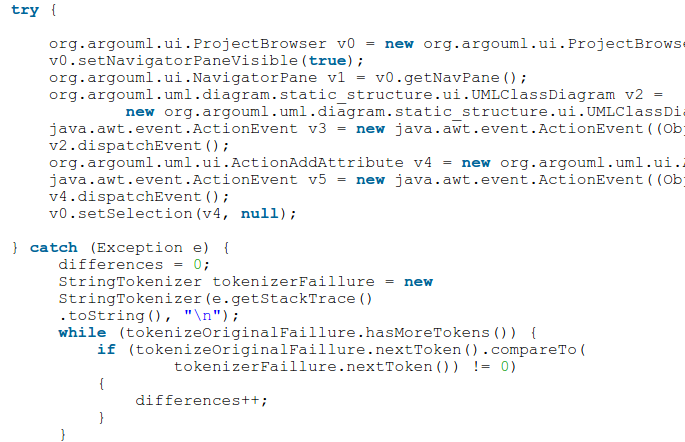
\includegraphics[width=0.97\linewidth]{media/testing2.png}
\end{figure}

\end{frame}

\begin{frame}
\frametitle{Experiments: Partially Reproduced Example}

\textbf{Jfreechart \#664}

\vspace{0.4cm} 

\textit{In ChartPanel.mouseMoved there's a line
of code which creates a new ChartMouseEvent using as first
parameter the object returned by getChart(). For getChart() is
legal to return null if the chart is null, but ChartMouseEvent's
constructor calls the parent constructor which throws an
IllegalArgumentException if the object passed in is null}

\vspace{0.4cm} 

\begin{small}
\texttt{1. java.lang.IllegalArgumentException: null source\\
2. at java.util.EventObject.<init>(
EventObject.java:38)\\
3. at\\
4 org.jfree.chart.ChartMouseEvent.<init>
(ChartMouseEvent.java:83)\\
5. at org.jfree.chart.ChartPanel
.mouseMoved(ChartPanel.java:1692)\\
\textbf{6. <deleted entry>}}
\end{small}

\end{frame}

\begin{frame}
\frametitle{Experiments: Not Reproduced Example}

\textbf{Log4j \#47957}

\vspace{0.4cm} 

\textit{Configure SyslogAppender with a Layout class that does not
exist; it throws a NullPointerException. Following is the
exception trace:}

\vspace{0.4cm} 

\begin{small}

\texttt{
1. 10052009 01:36:46 ERROR [Default: 1]
struts.CPExceptionHandler.execute
RID[(null;25KbxlK0voima4h00ZLBQFC;236Al8E60000045C3A
7D74272C4B4A61)]\\
2. Wrapping Exception in ModuleException\\
3. java.lang.NullPointerException\\
4. at org.apache.log4j.net.SyslogAppender
.append(SyslogAppender.java:250)\\
5. at org.apache.log4j.AppenderSkeleton
.doAppend(AppenderSkeleton.java:230)}

\end{small}

\end{frame}

\begin{frame}
\frametitle{Conclusion}

\begin{itemize}
\item JCHARMING (Java CrasH Automatic
Reproduction by directed Model checking)
\item Automatic bug
reproduction technique that combines crash traces and
directed model checking
\item Direct the model checking engine with a backward static slice
\item Was able to reproduce fully or partially 85\% (17/20) of the bugs
\vspace{0.5cm}
\item Stress JCHARMING with more bugs
\begin{itemize}
\item Fine tune the approach
\item Assess the scalability on larger / proprietary systems
\end{itemize}
\item Test the performances of JCHARMING with multi-threading related bugs


\end{itemize}

\end{frame}


%------------------------------------------------

\begin{frame}
\Huge{\centerline{QUESTIONS?}}
\end{frame}

%----------------------------------------------------------------------------------------

\end{document} 
